\documentclass[a4paper,11pt]{beamer}
\usepackage[utf8]{inputenc}
\usepackage{lmodern}
\usepackage{caption}
\usepackage{subcaption}
% Thème Darmstadt
\usetheme{Darmstadt}
\usepackage{graphicx}
\usepackage{caption}
\usepackage{ragged2e}
\usepackage{listings}
\usepackage{color}
\usepackage{gitdags}
\usepackage{fontawesome, wasysym}
%\captionsetup[figure]{labelformat=empty}

\setbeamertemplate{navigation symbols}{} 
\setbeamertemplate{footline} 
{  
	\begin{beamercolorbox}[ht=2.5ex,dp=1.125ex,%
      leftskip=.3cm,rightskip=.3cm plus1fil]{title in head/foot}%
      {\usebeamerfont{title in head/foot}\insertshorttitle} \hfill    
      \insertframenumber / \inserttotalframenumber%
    \end{beamercolorbox}%
%     \begin{beamercolorbox}[colsep=1.5pt]{lower separation line foot}
%     \end{beamercolorbox} 
}

% Informations sur la présentation
\title{Interface IAI}
\author{frank.buloup@univ-amu.fr} 
\institute{Institut des Sciences du Mouvement}
\date{}

\newcounter{exampleBlockCounter}
\setcounter{exampleBlockCounter}{1} 

\definecolor{comment}{rgb}{0.12, 0.38, 0.18 } %adjusted, in Eclipse: {0.25, 0.42, 0.30 } = #3F6A4D
\definecolor{keyword}{rgb}{0.37, 0.08, 0.25}  % #5F1441
\definecolor{string}{rgb}{0.06, 0.10, 0.98} % 

\lstset{
language=Python,
frame=single,
frameround=tttt,
rulesepcolor=\color{black},
showspaces=false,showtabs=false,tabsize=2,
numberstyle=\tiny,numbers=left,
stringstyle=\color{string},
keywordstyle = \color{keyword}\bfseries,
commentstyle=\color{comment}\itshape,
basicstyle=\ttfamily\footnotesize,
breaklines=true,
captionpos=b
}

%\includeonlyframes{current}

\begin{document}

% Première diapositive : Titre
\begin{frame}[plain]
    \titlepage
    \center{
\includegraphics[scale=0.75]{images/by-nc-sa.eps}}
 	\vspace{0.5cm}

	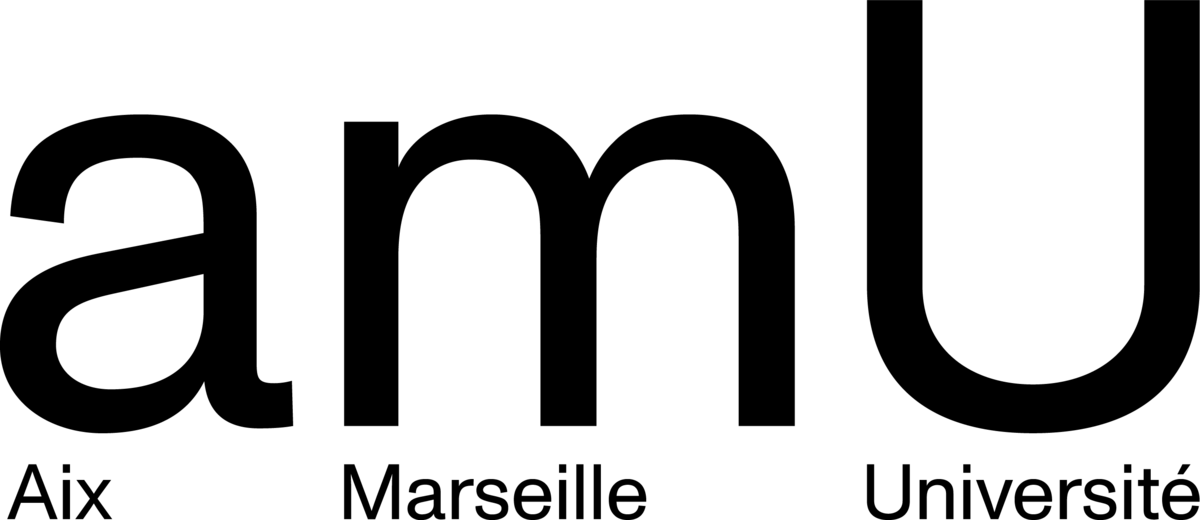
\includegraphics[scale=0.6]{images/LogoAMU.png}\hspace*{2cm}
	
\includegraphics[scale=0.35]{images/LogoCNRS.eps}\hspace*{2cm}
	
\includegraphics[scale=0.09]{images/LogoISM.eps}
    
\end{frame}

\begin{frame}{Interface IAI}
	\tableofcontents[hideallsubsections]
\end{frame}

\AtBeginSection{%
    \begin{frame}
        \tableofcontents[sections=\value{section}]
    \end{frame}
}

\section{Les différents éléments}
\subsection{Documentations}
\begin{frame}
\centering
	\textcolor{blue}{\textbf{\underline{\href{https://raw.githubusercontent.com/fbuloup/Interface_IAI/main/Documentation/RCS4-SLIDER(ME3769-1H).pdf}{Documentation actionneurs}}}}	
	
		\textcolor{blue}{\textbf{\underline{\href{https://raw.githubusercontent.com/fbuloup/Interface_IAI/main/Documentation/SCON-CB_CGB(ME0340-8A).pdf}{Documentation contrôleurs}}}}
\end{frame}
\subsection{Axe 0}
\begin{frame}
	\begin{block}{Actionneur : RCS4-SA7C-WA-200-24-200-T2-R03}
		\begin{itemize}
			\item Masse : 4.3kg
			\item Codeur absolu sans batterie - 200 watts
			\item Pas de la vis à bille (Ball Screw Lead) : 24mm par tour moteur
			\item Course totale : 200mm
			\item Vitesse maximale : 1500mm/s
			\item Force nominale en continu : 142N
			\item Codeur : 16384 impulsions par tour moteur
			\item Charge utile horizontale : 30kg - Charge utile verticale : 7kg
		\end{itemize}
	\end{block}
$$accuracy=\frac{BSL(mm)}{16384(pulses)}=\frac{24}{16384}=1.46\mu m$$	
$$Speed_{min}=\frac{BSL(mm)}{16384(pulses)}*1000(pulse/s)=\frac{24000}{16384}=1.46mm/pulse$$
\end{frame}
\begin{frame}
	\begin{block}{Contrôleur : SCON-CB-200WAI-PN-2-2}
		\begin{itemize}
			\item Type standard, 200 watts
			\item Codeur absolu/incrémental sans batterie
			\item Type PNP : type source de courant
			\item PIO de type PNP
			\item Commande par positionnement
			\item Commande par impulsions différentielles
		\end{itemize}
	\end{block}
\end{frame}

\subsection{Axe 1}
\begin{frame}
	\begin{block}{Actionneur : RCS4-SA8C-WA-400-30-200-T2-S}
		\begin{itemize}
			\item Masse : 5.6kg
			\item Codeur absolu sans batterie - 400 watts
			\item Pas de la vis à bille (Ball Screw Lead) : 30mm par tour moteur
			\item Course totale : 200mm
			\item Vitesse maximale : 1800mm/s
			\item Force nominale en continu : 226N
			\item Codeur : 16384 impulsions par tour moteur
			\item Charge utile horizontale : 30kg - Charge utile verticale : 12kg
		\end{itemize}
	\end{block}
$$accuracy=\frac{BSL(mm)}{16384(pulses)}=\frac{30}{16384}=1.83\mu m$$	
$$Speed_{min}=\frac{BSL(mm)}{16384(pulses)}*1000(pulse/s)=\frac{30000}{16384}=1.83mm/pulse$$
\end{frame}
\begin{frame}
	\begin{block}{Contrôleur : SCON-CB-400WAI-PN-2-2}
		\begin{itemize}
			\item Type standard, 400 watts
			\item Codeur absolu/incrémental sans batterie
			\item Type PNP : type source de courant
			\item PIO de type PNP
			\item Commande par positionnement
			\item Commande par impulsions différentielles
		\end{itemize}
	\end{block}
\end{frame}

\section{Interface avec un ADWinPro}
\subsection{Généralités}
\begin{frame}
	\begin{block}{Pulse et feedback}
		\begin{itemize}
			\item Commande par impulsion et non par positionnement
			\item Une carte par paire contrôleur/actionneur
			\item La commande sera faite avec des sorties DIO32 de l'ADwin
			\item La lecture du feedback sera faite avec une carte CO4-T
		\end{itemize}
	\end{block}
	\begin{block}{PIO}
		\begin{itemize}
			\item Le type PNP impose aussi une adaptation
			\item Une carte par paire contrôleur/actionneur
		\end{itemize}
	\end{block}
\end{frame}

\subsection{Carte Pulse/feedback}
\begin{frame}
	\centering
	\includegraphics[scale=0.33]{images/pcb.png}
\end{frame}

\begin{frame}
	\centering
	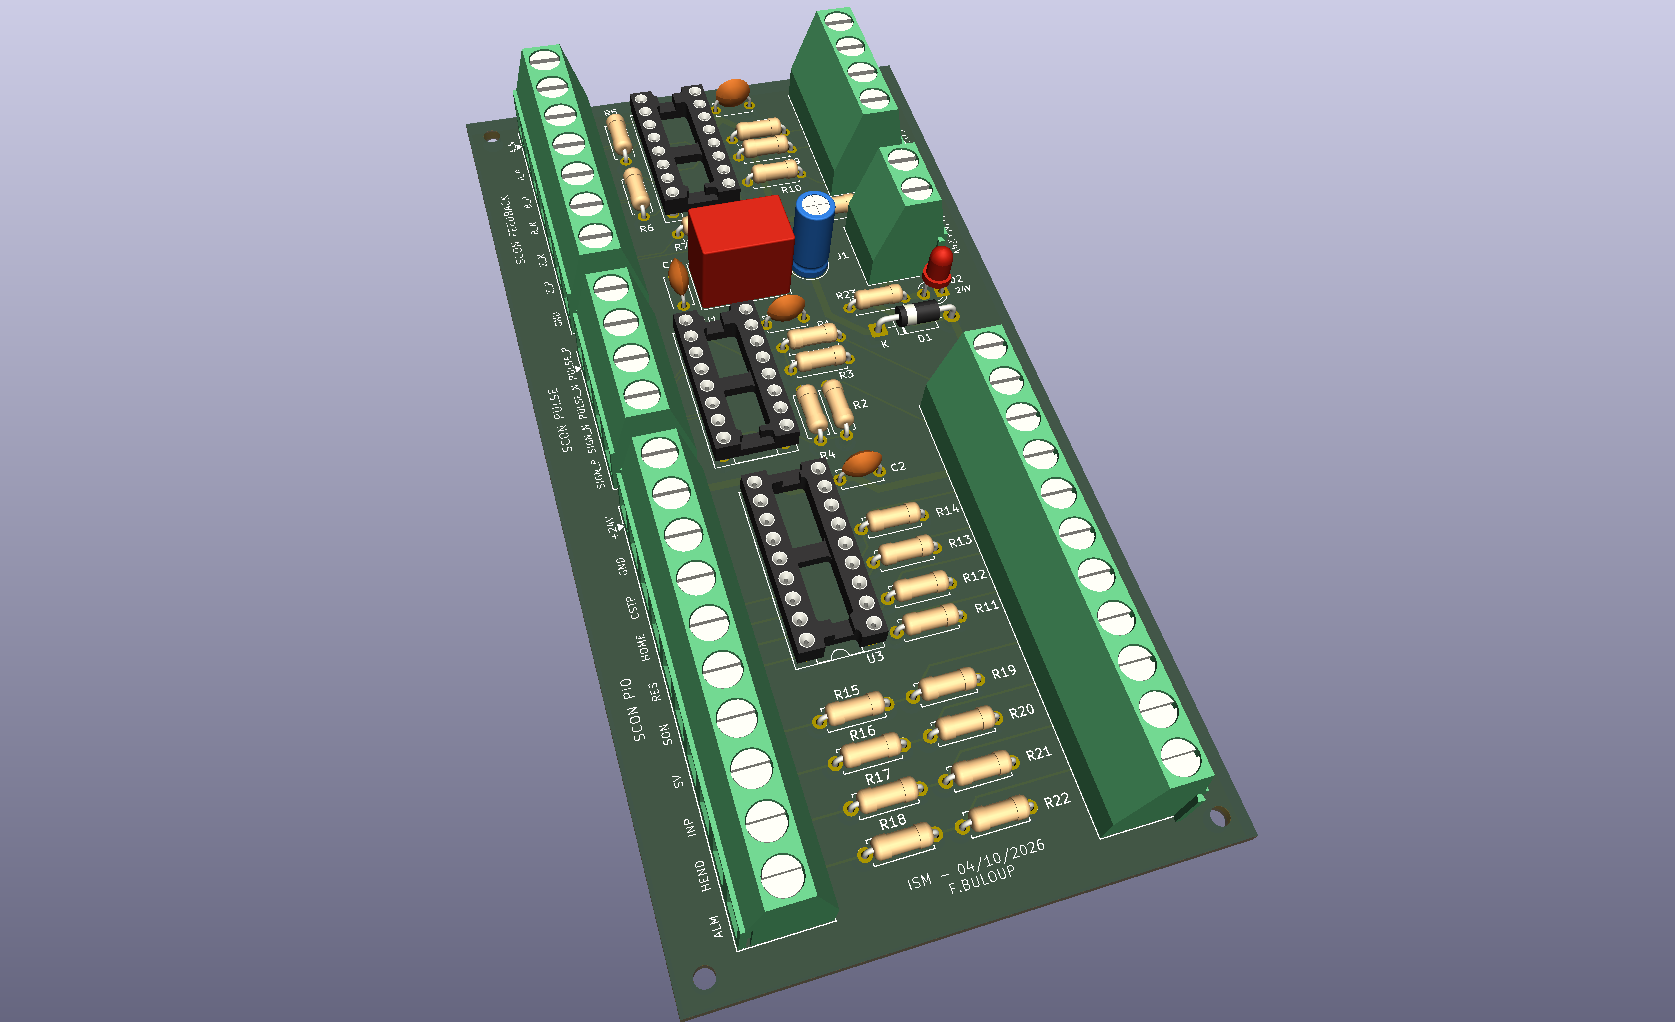
\includegraphics[scale=0.28]{images/Interface_IAI_1.png}
\end{frame}

\begin{frame}
	\centering
	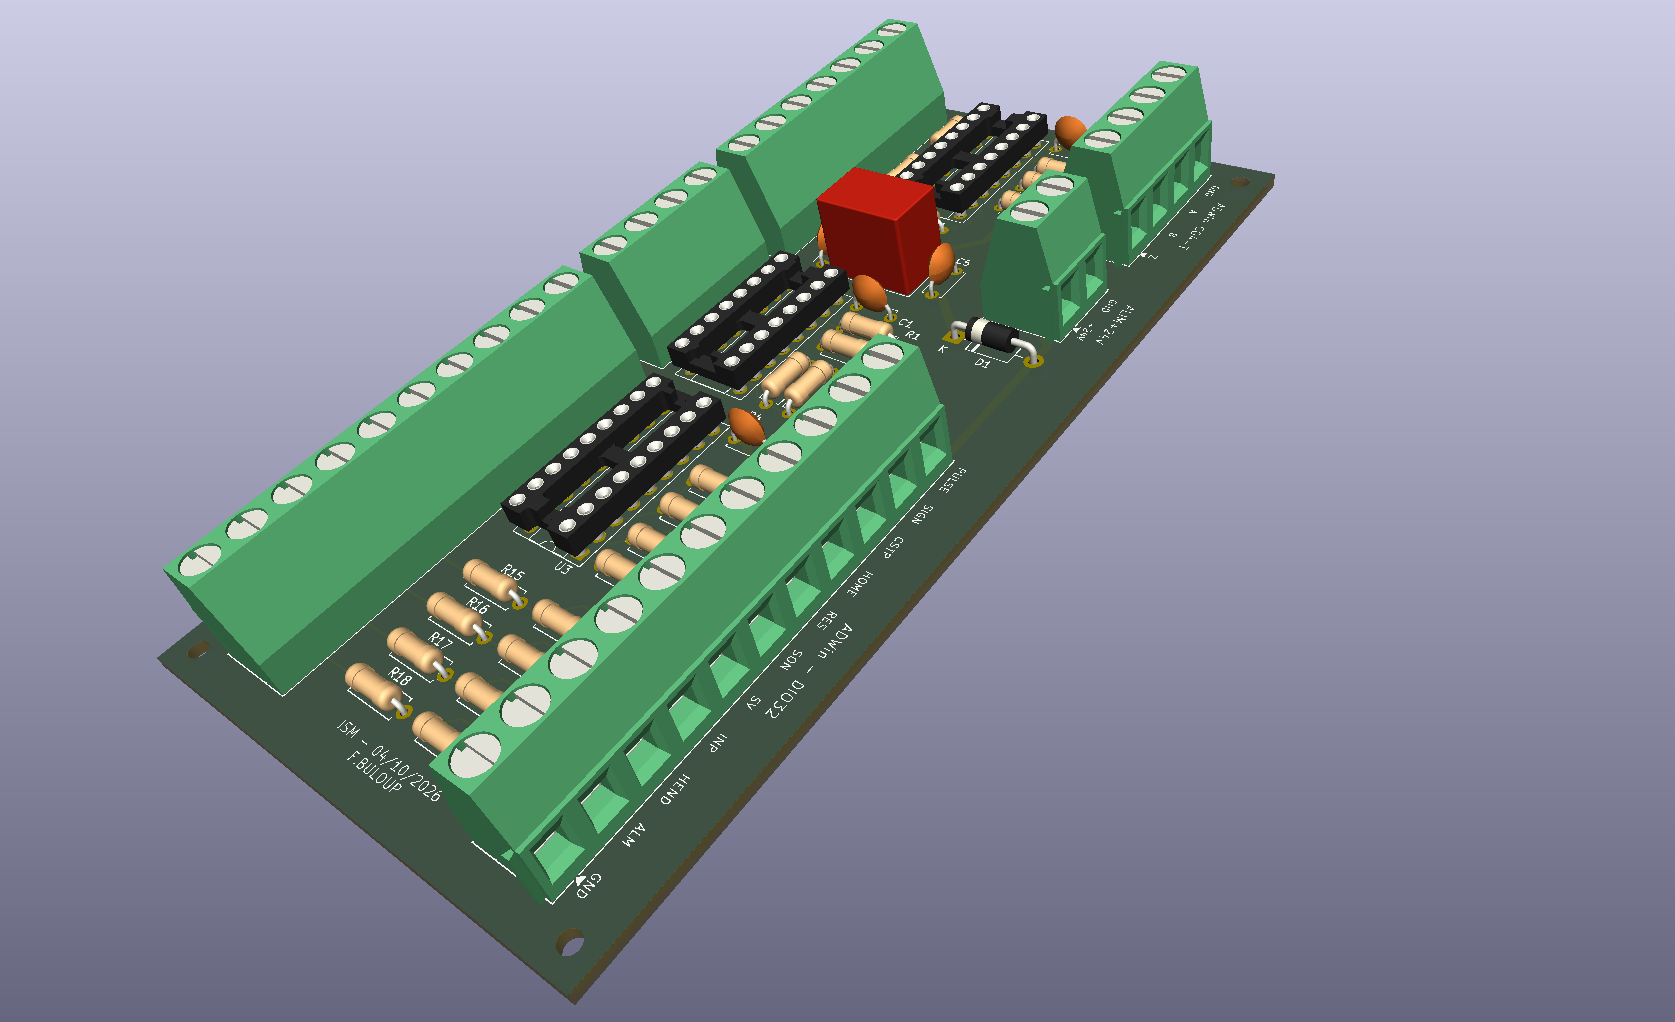
\includegraphics[scale=0.28]{images/Interface_IAI_2.png}
\end{frame}

\end{document}
